\section{Background}
\label{sec:bg}

\subsection{Simulation Ensembles}
Exploring parameter space of simulation models.
\begin{itemize}
    \item ParaGlide~\cite{Bergner13} is a visualization system designed for interactive exploration of parameter spaces of multidimensional simulation models. Provides an informative design study and characterization of the domain. It aims to help guide data generation using a region-based user interface for parameter sampling and then dividing the model's input parameter space into partitions that represent distinct output behavior. Input space partition is done as a Cartesian product of ranges in the various input dimensions. The work focus on multiple output or derived measures.
    
    \item He et al.~\cite{He2020} employed a neural network to support parameter space exploration for ensemble simulations that are visualized in situ. They developed a convolutional regression model to learn a mapping from simulation and visualization parameters to visualization results. With the trained model, users can generate new images for different simulation parameters under various visualization settings. The work focuses on synthesizing images rather than of direct analysis of the the data
\end{itemize}

\subsubsection{Visual Steering}
\cite{Matkovic14, Splechtna15, Matkovic18}

\subsection{Topological Analysis}
Chazal~\cite{Chazal11}

\subsection{Morse Theory}
\label{sec:morse}
Morse~\cite{morse63}, Timo~\cite{Timo04}

Merge trees: expand. Giving a value, a merge tree can be used to extract a level set or segment the data but removing all the points below the given value. Merge trees were also used for visual exploration.

\subsection{Morse-Smale Approximation}
\label{sec:morse-smale}
Edelsbrunner~\cite{Edelsbrunner03}


\subsection{Visual Exploration}
\label{sec:hd-exploration}

\begin{itemize}
    \item Gerber 2010 work (this work is based on it). 
    \begin{itemize}
        \item Fit an inverse regression curve in each crystal to provide some sort of geometric summary. The curves are 1d curves in $R^d$ and in order to display them, Gerber project the curves down to 3d based on a PCA of all the data points.
        
        \item Once the user selects a persistence value using (\autoref{fig:persistence-ui}),  Gerber extracts the Morse-Smale representation of the data and then display all the inverse curves (see \autoref{sec:curve-fitting}) for in the partitions (crystals) in the 3D view.
        
        \item The 3D is problematic because 
            \begin{itemize}
                \item confusing - the axis are not clear and the twists in the curves don't provide any meaningful info
                \item to be meaningful the curves suppose to meet at the ends, which require some fiddling with the data. 
                \item the curves are not a good representation for coarse partitions that do not have a good linear model. 
            \end{itemize}
        
        \item the user can see details only about a single partition at a time
        
        \item single global refinement (persistence) level based on \autoref{fig:persistence-ui}
    
    \end{itemize}

    \item Dan's works. 
    \begin{itemize}
        \item Dan uses only linear lines instead of inverse regression curves because they are too expensive to precompute as Gerber did
        \item explain the views
        \item what are important aspects should be outlined here?
    \end{itemize}
    
    \item Use a persistence diagram \cite{Cohen-Steiner07}. Provides overall view of a MSC/MS but without connectivity between points. Does not address hierarchical MSC approximations.
\end{itemize}


\begin{figure}[htb]
    \begin{center}
     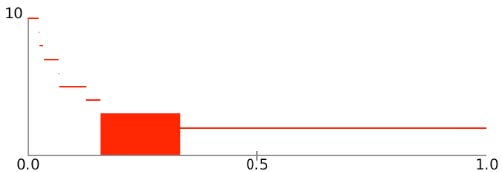
\includegraphics[width=\linewidth]{persistence-ui}
    \caption{Persistence curve showing the number of partitions as a function of persistence.}
    \label{fig:persistence-ui}
    \end{center}
\end{figure}


    \caption{Persistence curve showing the number of partitions as a function of persistence.}

